\chapter{Data-driven Surrogates for Parabolic Two-Temperature Model Damage Threshold Prediction in Metals}
\label{ch:regression}

\section{Introduction}

The previous chapters established the physical and numerical setting for two-temperature modelling of ultrashort laser heating in metallic films. Direct finite-difference pTTM simulations remain the reference calculation in this chapter, but repeated forward solves become expensive when fluence, optical response, thermophysical parameters, and film geometry must be explored over a broad domain. The purpose of the present chapter is therefore to formulate a data-driven surrogate framework for the maximum lattice-temperature response and for the damage-threshold fluence inferred from that response.

This chapter contains two complementary surrogate studies. The first is a two-dimensional linear pTTM surrogate study, in which a filtered synthetic response dataset is used to train LightGBM and residual MLP regressors. The second is a nonlinear two-dimensional pTTM extension at the \(\num{20000}\) accepted-sample scale, using temperature-dependent \(C_e(T_e)\) and \(G(T_e)\), Lorentz--Drude optical descriptors, and source-term-informed feature engineering. In both studies, the surrogate target is the maximum lattice temperature \(T_{l,\max}\), and damage-threshold fluences are obtained by inverting predicted temperature--fluence responses. The nonlinear analysis is included at a smaller accepted-sample scale than the linear study, and large-scale nonlinear datasets remain future work.

\section{Synthetic two-dimensional linear pTTM dataset}

The linear surrogate dataset is generated from a two-dimensional explicit pTTM with constant $C_e$, $C_l$, $G$, and scalar optical-source parameters. In the notation of this chapter, the sampled input vector is
\begin{equation}
    \boldsymbol{\theta}_{\mathrm{lin}}
    =
    \left(
    F, C_e, C_l, G, k_{e0}, L_b, \alpha, R, \lambda, h
    \right),
\end{equation}
where $F$ is the incident fluence, $C_e$ and $C_l$ are the electron and lattice heat capacities, $G$ is the electron-phonon coupling factor, $k_{e0}$ is the electron conductivity scale, $L_b$ is the ballistic length, $\alpha$ is the absorption coefficient, $R$ is the reflectivity, $\lambda$ is the laser wavelength, and $h$ is the film thickness.

The lattice conductivity is not sampled independently. The linear dataset uses the fixed convention
\begin{equation}
    k_l=0.01\,k_{e0}.
\end{equation}
For a sampled parameter vector, the numerical solver advances the coupled electron and lattice temperatures and records scalar response quantities. The sampled ranges used for the two-dimensional linear pTTM study are listed in Table~\ref{tab:ch4-linear-sampled-variables}.

\begin{table}[htbp]
    \centering
    \caption{Sampled variables for the two-dimensional linear pTTM surrogate dataset.}
    \label{tab:ch4-linear-sampled-variables}
    \small
    \begin{tabular}{lllll}
\hline
Variable & Meaning & Range & Sampling & Units \\
\hline
$F$ & Laser fluence & $[10,40000]$ & log-LHS & J\,m$^{-2}$ \\
$C_e$ & Electron heat capacity & $[10^4,2\times10^6]$ & log-LHS & J\,m$^{-3}$\,K$^{-1}$ \\
$C_l$ & Lattice heat capacity & $[1.5\times10^6,5\times10^6]$ & linear-LHS & J\,m$^{-3}$\,K$^{-1}$ \\
$G$ & Electron-phonon coupling & $[10^{16},5\times10^{18}]$ & log-LHS & W\,m$^{-3}$\,K$^{-1}$ \\
$k_{e0}$ & Electron conductivity scale & $[20,500]$ & log-LHS & W\,m$^{-1}$\,K$^{-1}$ \\
$L_b$ & Ballistic length & $[10^{-9},1.5\times10^{-7}]$ & log-LHS & m \\
$\alpha$ & Absorption coefficient & $[10^7,5\times10^8]$ & log-LHS & m$^{-1}$ \\
$R$ & Reflectivity & $[0.5,0.999]$ & linear-LHS & dimensionless \\
$\lambda$ & Wavelength & $[1000,1400]$ & linear-LHS & nm \\
$h$ & Film thickness & $[2\times10^{-7},10^{-6}]$ & log-LHS & m \\
\hline
\end{tabular}

\end{table}

\begin{algorithm}[htbp]
    \caption{Accepted synthetic sample generation for the linear pTTM surrogate dataset}
    \label{alg:ch4-linear-data-generation}
    \begin{algorithmic}[1]
        \Require Requested sample count $N$, parameter domain $\Theta_{\mathrm{lin}}$, numerical pTTM solver $\mathcal{S}$, acceptance rule $\mathcal{A}$
        \Ensure Accepted dataset $\mathcal{D}$
        \State Initialise $\mathcal{D}\gets\emptyset$ and attempt counter $a\gets0$
        \While{$|\mathcal{D}|<N$ and the attempt budget is not exhausted}
        \State Draw a candidate input vector $\boldsymbol{\theta}^{(a)}\sim p(\boldsymbol{\theta})$
        \State Evaluate the numerical response $\mathbf{o}^{(a)}\gets\mathcal{S}(\boldsymbol{\theta}^{(a)})$
        \If{$\mathcal{A}(\boldsymbol{\theta}^{(a)},\mathbf{o}^{(a)})$ is satisfied}
        \State Compute $y^{(a)}=T_{l,\max}^{(a)}$
        \State Append $(\boldsymbol{\theta}^{(a)},y^{(a)},\mathbf{o}^{(a)})$ to $\mathcal{D}$
        \Else
        \State Record the rejection reason
        \EndIf
        \State $a\gets a+1$
        \EndWhile
        \State \Return $\mathcal{D}$
    \end{algorithmic}
\end{algorithm}

\section{Sampling, filtering, and target definition}

For a numerical pTTM solve, let $T_l(\mathbf{x},t;\boldsymbol{\theta})$ denote the lattice-temperature field. The scalar target used for the linear surrogate is
\begin{equation}
    T_{l,\max}(\boldsymbol{\theta})
    =
    \max_{\mathbf{x},t}T_l(\mathbf{x},t;\boldsymbol{\theta}).
\end{equation}
Writing $y_i=T_{l,\max}(\boldsymbol{\theta}_i)$, the accepted training set is
\begin{equation}
    \mathcal{D}_{\mathrm{acc}}
    =
    \left\{
    \left(\boldsymbol{\theta}_i,y_i\right):
    y_i<\infty,\;
    y_i\leq 10^4\,\mathrm{K}
    \right\}.
\end{equation}
The upper target filter is a modelling and training-data policy rather than a physical melting criterion. It removes non-finite solves and high-temperature responses that would otherwise dominate the single-target regression loss. This stabilises the first surrogate-learning problem, but it also censors the response tail and must be kept visible when interpreting high-temperature material cases.

\begin{figure}[htbp]
    \centering
    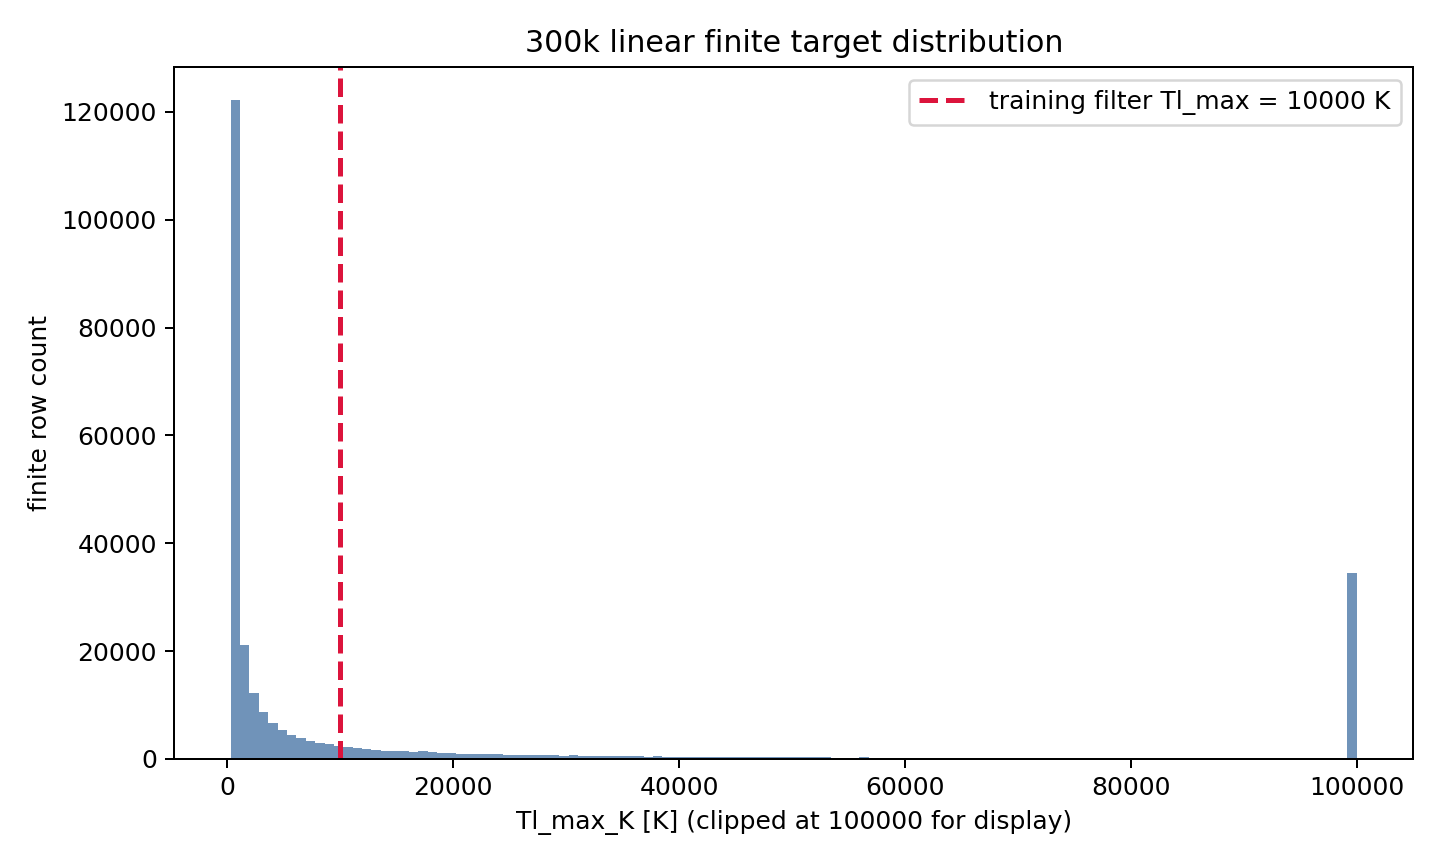
\includegraphics[width=0.82\textwidth]{figures/ch4/linear_ttm/target_distribution_filter.png}
    \caption{Distribution of finite $T_{l,\max}$ values in the linear pTTM sweep with the $T_{l,\max}=\SI{10000}{\kelvin}$ training filter indicated.}
    \label{fig:ch4-target-filter}
\end{figure}

\begin{figure}[htbp]
    \centering
    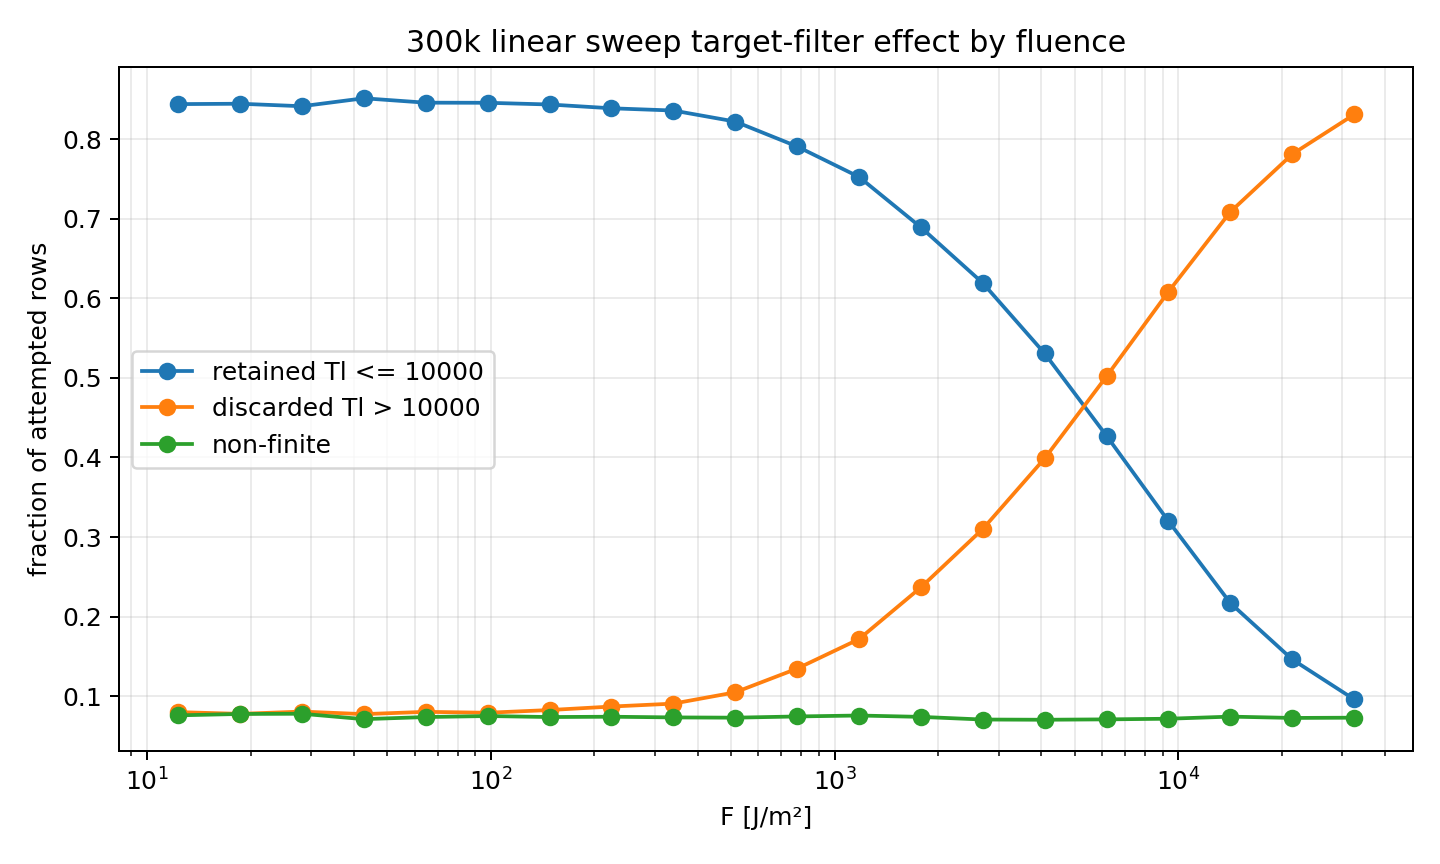
\includegraphics[width=0.82\textwidth]{figures/ch4/linear_ttm/retained_discarded_vs_fluence.png}
    \caption{Retained, high-temperature discarded, and non-finite sample fractions as a function of fluence under the $T_{l,\max}\leq\SI{10000}{\kelvin}$ filter.}
    \label{fig:ch4-filter-vs-fluence}
\end{figure}

\section{Surrogate-learning formulation}

The surrogate-learning task is to approximate the numerical map
\begin{equation}
    f:\boldsymbol{\theta}\mapsto T_{l,\max}.
\end{equation}
Given $\mathcal{D}_{\mathrm{acc}}=\{(\boldsymbol{\theta}_i,y_i)\}_{i=1}^{N}$, a model family $\mathcal{F}$, and a hyperparameter vector $\boldsymbol{\eta}$, training minimises the empirical squared-error objective
\begin{equation}
    \hat{f}_{\boldsymbol{\eta}}
    =
    \arg\min_{f\in\mathcal{F}_{\boldsymbol{\eta}}}
    \frac{1}{N_{\mathrm{tr}}}
    \sum_{i\in\mathcal{I}_{\mathrm{tr}}}
    \left[
        f(\boldsymbol{\theta}_i)-y_i
        \right]^2.
\end{equation}
Model selection uses validation RMSE,
\begin{equation}
    \mathrm{RMSE}_{\mathrm{val}}(\boldsymbol{\eta})
    =
    \left[
    \frac{1}{N_{\mathrm{val}}}
    \sum_{i\in\mathcal{I}_{\mathrm{val}}}
    \left(
    \hat{f}_{\boldsymbol{\eta}}(\boldsymbol{\theta}_i)-y_i
    \right)^2
    \right]^{1/2},
\end{equation}
and final reporting uses the same RMSE definition on the held-out test set, together with mean absolute error and $R^2$.

Residual-calibrated predictive intervals are formed from held-out surrogate residuals. For residuals
\begin{equation}
    r_i
    =
    y_i-\hat{f}(\boldsymbol{\theta}_i),
    \qquad i\in\mathcal{I}_{\mathrm{test}},
\end{equation}
let $q_{\gamma}$ be the empirical $\gamma$ quantile of $\{|r_i|\}$. The symmetric predictive band for a new input is
\begin{equation}
    \mathcal{I}_{\gamma}(\boldsymbol{\theta})
    =
    \left[
    \hat{f}(\boldsymbol{\theta})-q_{\gamma},
    \hat{f}(\boldsymbol{\theta})+q_{\gamma}
    \right].
\end{equation}
These intervals quantify surrogate error relative to the numerical linear pTTM target. They do not include numerical discretisation uncertainty, material-parameter uncertainty, or cross-model discrepancy with nonlinear reference calculations.

\section{Surrogate models and hyperparameter selection}

The first surrogate family is LightGBM, treated here as a gradient-boosted decision-tree regressor for heterogeneous tabular inputs \cite{Friedman_2001,ke2017lightgbm}. Gradient boosting builds an additive ensemble by fitting successive trees to reduce the current prediction error, which makes it suitable for nonlinear interactions among physical parameters with different units and scales. The second family is a residual multilayer perceptron. It maps standardised inputs through fully connected residual blocks and predicts the scalar target $T_{l,\max}$ with a final regression head \cite{goodfellow2016deep}.

For the linear surrogate study, hyperparameters are selected by validation-RMSE optimisation using Optuna \cite{akiba2019optuna}. Each trial proposes a hyperparameter vector $\boldsymbol{\eta}$, trains a candidate model on the training subset, evaluates $\mathrm{RMSE}_{\mathrm{val}}(\boldsymbol{\eta})$, and selects
\begin{equation}
    \boldsymbol{\eta}^{\star}
    =
    \arg\min_{\boldsymbol{\eta}}
    \mathrm{RMSE}_{\mathrm{val}}(\boldsymbol{\eta}).
\end{equation}
The test subset is not used for hyperparameter selection. It is reserved for the final held-out synthetic performance report. This Optuna procedure applies to the linear surrogate study. The nonlinear \(\num{20000}\)-sample analysis uses fixed bounded LightGBM and MLP configurations, and no full nonlinear Optuna run was performed.

\begin{algorithm}[htbp]
    \caption{Surrogate training and validation-based model selection}
    \label{alg:ch4-surrogate-training}
    \begin{algorithmic}[1]
        \Require Accepted dataset $\mathcal{D}_{\mathrm{acc}}$, model family $\mathcal{F}$, hyperparameter search space $\mathcal{H}$
        \Ensure Selected surrogate $\hat{f}$
        \State Split $\mathcal{D}_{\mathrm{acc}}$ into training, validation, and test subsets
        \For{each hyperparameter proposal $\boldsymbol{\eta}\in\mathcal{H}$}
        \State Train $\hat{f}_{\boldsymbol{\eta}}$ on the training subset
        \State Compute $\mathrm{RMSE}_{\mathrm{val}}(\boldsymbol{\eta})$ on the validation subset
        \EndFor
        \State Select $\boldsymbol{\eta}^{\star}\gets\arg\min_{\boldsymbol{\eta}}\mathrm{RMSE}_{\mathrm{val}}(\boldsymbol{\eta})$
        \State Retain or retrain the best model according to the selected protocol
        \State Evaluate $\hat{f}_{\boldsymbol{\eta}^{\star}}$ on the held-out test subset
        \State \Return $\hat{f}_{\boldsymbol{\eta}^{\star}}$
    \end{algorithmic}
\end{algorithm}

\section{Synthetic held-out performance}

The linear pTTM sweep comprised \(\num{300000}\) requested samples. Of these, \(\num{277914}\) rows produced finite $T_{l,\max}$ values and \(\num{22086}\) rows were non-finite. Among the finite rows, \(\num{82857}\) exceeded the $T_{l,\max}=\SI{10000}{\kelvin}$ training cap, leaving \(\num{195057}\) retained rows after the combined finite-response and high-temperature filter. The retained dataset was split into \(\num{156045}\) training rows, \(\num{19506}\) validation rows, and \(\num{19506}\) held-out test rows.

The held-out synthetic metrics in Table~\ref{tab:ch4-heldout-metrics} show that both surrogate families learn the retained filtered numerical target well. The residual MLP is stronger on this target, with an RMSE of $\SI{115.190}{\kelvin}$ and $R^2=0.997264$, compared with the LightGBM RMSE of $\SI{215.230}{\kelvin}$ and $R^2=0.990449$. These figures assess interpolation within the accepted target policy. They do not assess accuracy in the censored high-temperature tail removed by the $T_{l,\max}\leq\SI{10000}{\kelvin}$ rule.

\begin{table}[htbp]
    \centering
    \caption{Held-out synthetic test metrics for the linear pTTM surrogate study.}
    \label{tab:ch4-heldout-metrics}
    \begin{tabular}{lrrrr}
        \toprule
        Model        & Test rows & RMSE (K) & MAE (K) & $R^2$    \\
        \midrule
        LightGBM     & 19506     & 215.230  & 101.653 & 0.990449 \\
        Residual MLP & 19506     & 115.190  & 20.062  & 0.997264 \\
        \bottomrule
    \end{tabular}
\end{table}

\begin{figure}[htbp]
    \centering
    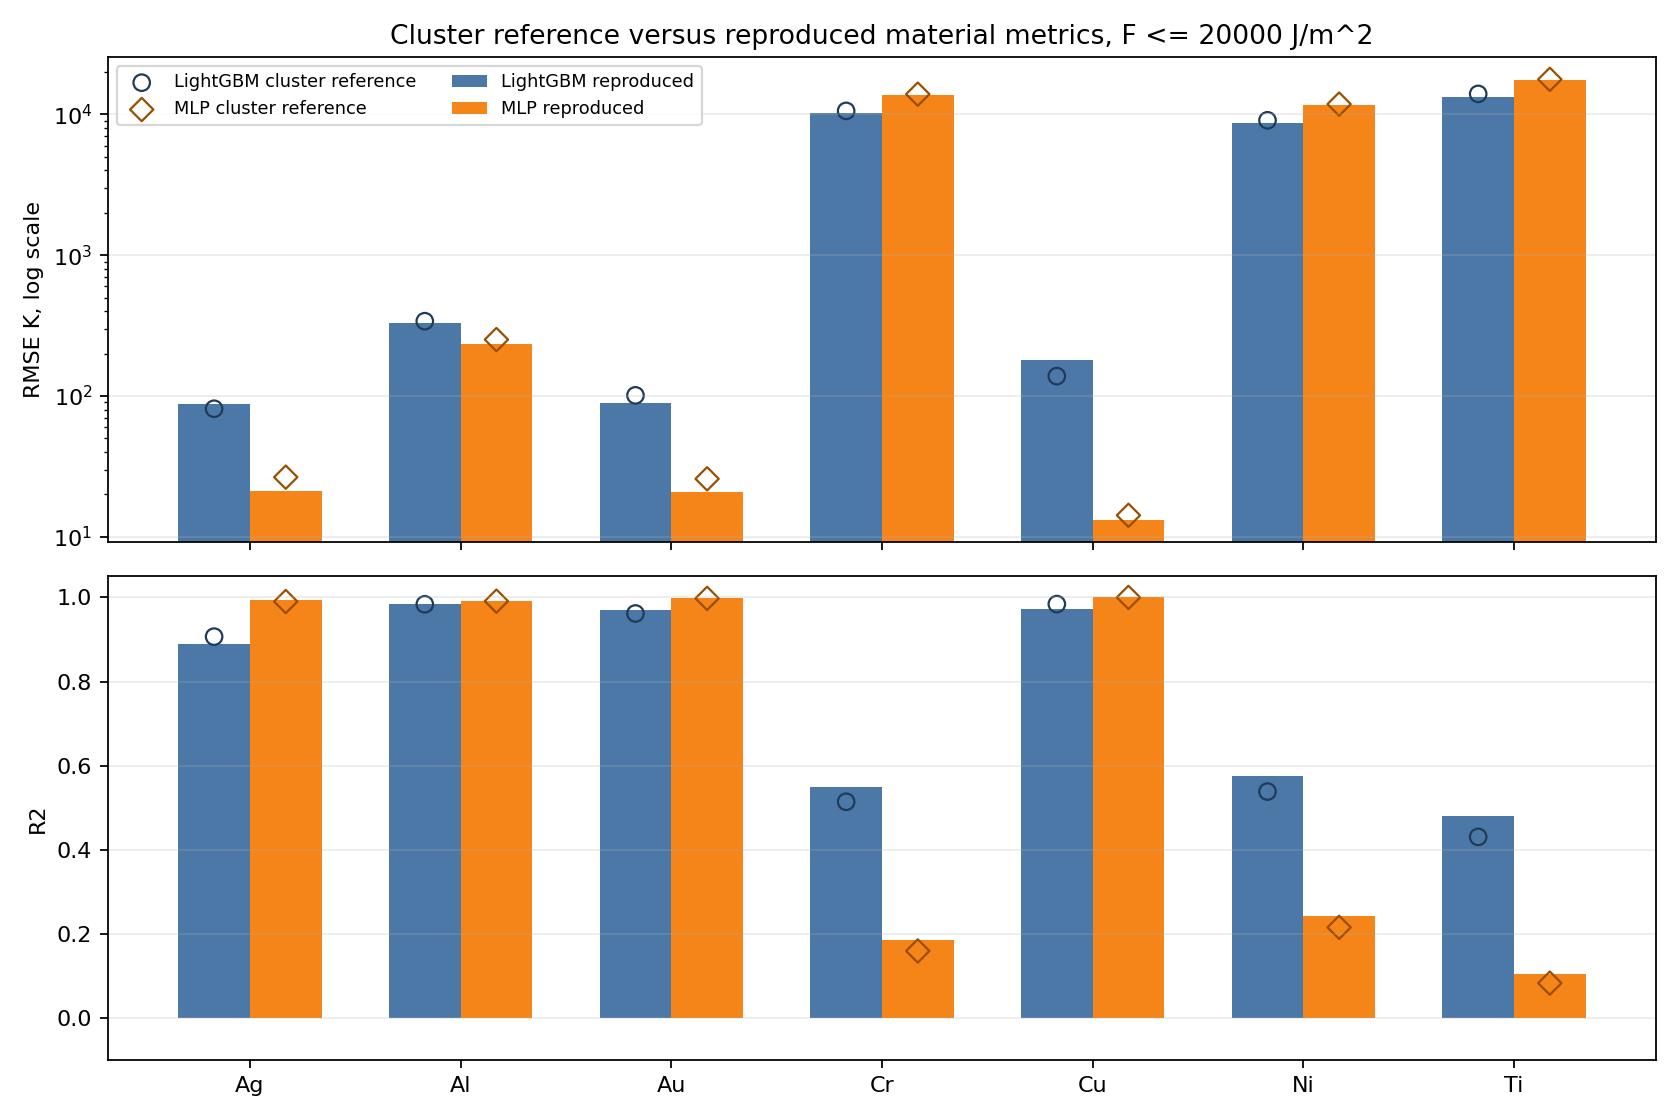
\includegraphics[width=0.86\textwidth]{figures/ch4/linear_ttm/model_metric_comparison.png}
    \caption{Compact comparison of surrogate validation metrics for the two-dimensional linear pTTM target.}
    \label{fig:ch4-model-metric-comparison}
\end{figure}

\section{Real-material validation and threshold inversion}

Real-material validation evaluates the trained surrogates on material-specific fluence curves and compares them with the numerical two-dimensional linear pTTM response. For a fixed material and fixed non-fluence parameters, the melting-threshold fluence is defined as
\begin{equation}
    F_{\mathrm{th}}
    =
    \inf\left\{
    F:
    T_{l,\max}(F)\geq T_{\mathrm{melt}}
    \right\}.
\end{equation}
For a discrete fluence curve, the first bracketing pair satisfies
\begin{equation}
    T_{l,\max}(F_a)
    <
    T_{\mathrm{melt}}
    \leq
    T_{l,\max}(F_b),
    \qquad
    F_a<F_b.
\end{equation}
The reported threshold uses linear interpolation in $\log_{10}F$,
\begin{equation}
    \log_{10}F_{\mathrm{th}}
    =
    \log_{10}F_a
    +
    \frac{
    T_{\mathrm{melt}}-T_{l,\max}(F_a)
    }{
    T_{l,\max}(F_b)-T_{l,\max}(F_a)
    }
    \left(
    \log_{10}F_b-\log_{10}F_a
    \right),
\end{equation}
followed by $F_{\mathrm{th}}=10^{\log_{10}F_{\mathrm{th}}}$.

\begin{algorithm}[htbp]
    \caption{Damage-threshold inversion in logarithmic fluence}
    \label{alg:ch4-threshold-inversion}
    \begin{algorithmic}[1]
        \Require Fluence grid $\{F_k\}_{k=1}^{K}$, temperature curve $\{\hat{T}_{l,\max}(F_k)\}_{k=1}^{K}$, melting temperature $T_{\mathrm{melt}}$
        \Ensure Threshold estimate $F_{\mathrm{th}}$ or no-crossing status
        \State Sort the curve by increasing $F_k$
        \For{$k=1,\ldots,K-1$}
        \If{$\hat{T}_{l,\max}(F_k)<T_{\mathrm{melt}}\leq\hat{T}_{l,\max}(F_{k+1})$}
        \State Set $F_a\gets F_k$, $F_b\gets F_{k+1}$
        \State Set $T_a\gets\hat{T}_{l,\max}(F_a)$ and $T_b\gets\hat{T}_{l,\max}(F_b)$
        \State Interpolate $\log_{10}F_{\mathrm{th}}$ between $(F_a,T_a)$ and $(F_b,T_b)$
        \State \Return $F_{\mathrm{th}}\gets10^{\log_{10}F_{\mathrm{th}}}$
        \EndIf
        \EndFor
        \State \Return no crossing in the sampled fluence interval
    \end{algorithmic}
\end{algorithm}

Material-validation metrics for the supplied fluence interval $F\leq\SI{20000}{\joule\per\metre\squared}$ are summarised in Table~\ref{tab:ch4-material-metrics}. The noble-metal cases Ag, Au, and Cu are well supported by the retained linear surrogate manifold and are predicted accurately, especially by the residual MLP. Aluminium remains reasonable but less accurate than the best-supported noble-metal cases. By contrast, Cr, Ni, and Ti show severe high-temperature errors. These failures should not be described as pure fluence extrapolation, because the sampled fluence domain extends to $\SI{40000}{\joule\per\metre\squared}$; they instead indicate that the retained target policy and the material-regime support are insufficient for those high-temperature curves. The nonlinear analysis below revisits the Ni and Ti interpretation after temperature-dependent \(C_e(T_e)\) and \(G(T_e)\) are included.

\begin{table}[htbp]
    \centering
    \caption{Material-validation metrics for $F\leq\SI{20000}{\joule\per\metre\squared}$. RMSE values are in kelvin.}
    \label{tab:ch4-material-metrics}
    \small
    \begin{tabular}{lrrrr}
        \toprule
        Material & LightGBM RMSE & LightGBM $R^2$ & MLP RMSE & MLP $R^2$ \\
        \midrule
        Ag       & 88.4          & 0.8890         & 21.3     & 0.9936    \\
        Al       & 328.8         & 0.9844         & 235.1    & 0.9920    \\
        Au       & 88.8          & 0.9703         & 20.8     & 0.9984    \\
        Cr       & 10190.8       & 0.5493         & 13694.2  & 0.1861    \\
        Cu       & 180.7         & 0.9725         & 13.3     & 0.9999    \\
        Ni       & 8687.3        & 0.5767         & 11614.5  & 0.2433    \\
        Ti       & 13356.5       & 0.4795         & 17503.4  & 0.1060    \\
        \bottomrule
    \end{tabular}
\end{table}

External cross-model threshold values are omitted from the public source pending documented redistribution terms. The internal numerical and surrogate estimates reported below remain distinct from any external calculation.

\begin{table}[htbp]
    \centering
    \caption{Damage-threshold estimates with residual-calibrated 95\% surrogate intervals. Values are shown in \si{\kilo\joule\per\metre\squared}.}
    \label{tab:ch4-threshold-intervals}
    \scriptsize
    \begin{tabular}{lrrrrrrr}
        \toprule
        Material & Linear & LightGBM & LGBM low & LGBM high & MLP    & MLP low & MLP high \\
        \midrule
        Ag       & 15.211 & 15.129   & 9.939    & 19.370    & 14.140 & 13.121  & 15.205   \\
        Au       & 8.755  & 9.901    & 6.693    & 13.982    & 8.363  & 7.781   & 8.952    \\
        Cu       & 4.228  & 4.107    & 2.703    & 5.714     & 4.228  & 3.938   & 4.509    \\
        Ni       & 0.472  & 0.444    & 0.341    & 0.622     & 0.479  & 0.455   & 0.503    \\
        Ti       & 0.392  & 0.442    & 0.331    & 0.523     & 0.388  & 0.371   & 0.405    \\
        \bottomrule
    \end{tabular}
\end{table}

\begin{figure}[htbp]
    \centering
    \PublicExternalValuesOmitted[0.82\textwidth]
    \caption{Threshold estimates from the numerical linear pTTM solver and the two surrogates, with residual-calibrated intervals. External comparison values are omitted from the public source.}
    \label{fig:ch4-threshold-intervals}
\end{figure}

The internal threshold estimates in Table~\ref{tab:ch4-threshold-intervals} are consistent with the material-validation pattern. External comparison values are deliberately excluded from the public source and are not interpreted as direct surrogate residuals.

\section{High-temperature limitation analysis}

The $T_{l,\max}\leq\SI{10000}{\kelvin}$ filter is both a useful training-data policy and a limitation. It prevents the single-target loss from being dominated by extreme high-temperature or unstable responses, but it also removes the part of the response manifold that some real-material fluence curves enter within the validation interval. Figures~\ref{fig:ch4-target-filter} and~\ref{fig:ch4-filter-vs-fluence} therefore define an essential boundary condition on the interpretation of all reported surrogate errors.

The material-level crossings of the $\SI{10000}{\kelvin}$ cap make this limitation explicit. Cr crosses the cap at approximately $2824.484\,\mathrm{J\,m^{-2}}$, Ni at $3211.256\,\mathrm{J\,m^{-2}}$, and Ti at $2316.526\,\mathrm{J\,m^{-2}}$. These crossings occur well inside the $F\leq\SI{20000}{\joule\per\metre\squared}$ validation window. Aluminium crosses much later, at approximately $16265.830\,\mathrm{J\,m^{-2}}$. Ag and Au do not cross within the same validation window, while the Cu crossing occurs at approximately $39267.560\,\mathrm{J\,m^{-2}}$, outside the $F\leq\SI{20000}{\joule\per\metre\squared}$ material-validation window.

Figure~\ref{fig:ch4-material-feature-support} gives a complementary support diagnostic by locating the real-material parameter values inside the retained synthetic training distribution. Each entry is the percentile position of a real-material parameter after the finite-response and $T_{l,\max}\leq\SI{10000}{\kelvin}$ filter. The heatmap does not by itself prove an out-of-distribution failure, but it shows that the difficult transition-metal cases combine high-temperature target censoring with less favourable retained-manifold support in conductivity, coupling, and optical-response coordinates. The corresponding selected material-parameter values are collected in Appendix~\ref{app:ch4-sampling-support}.

\begin{figure}[htbp]
    \centering
    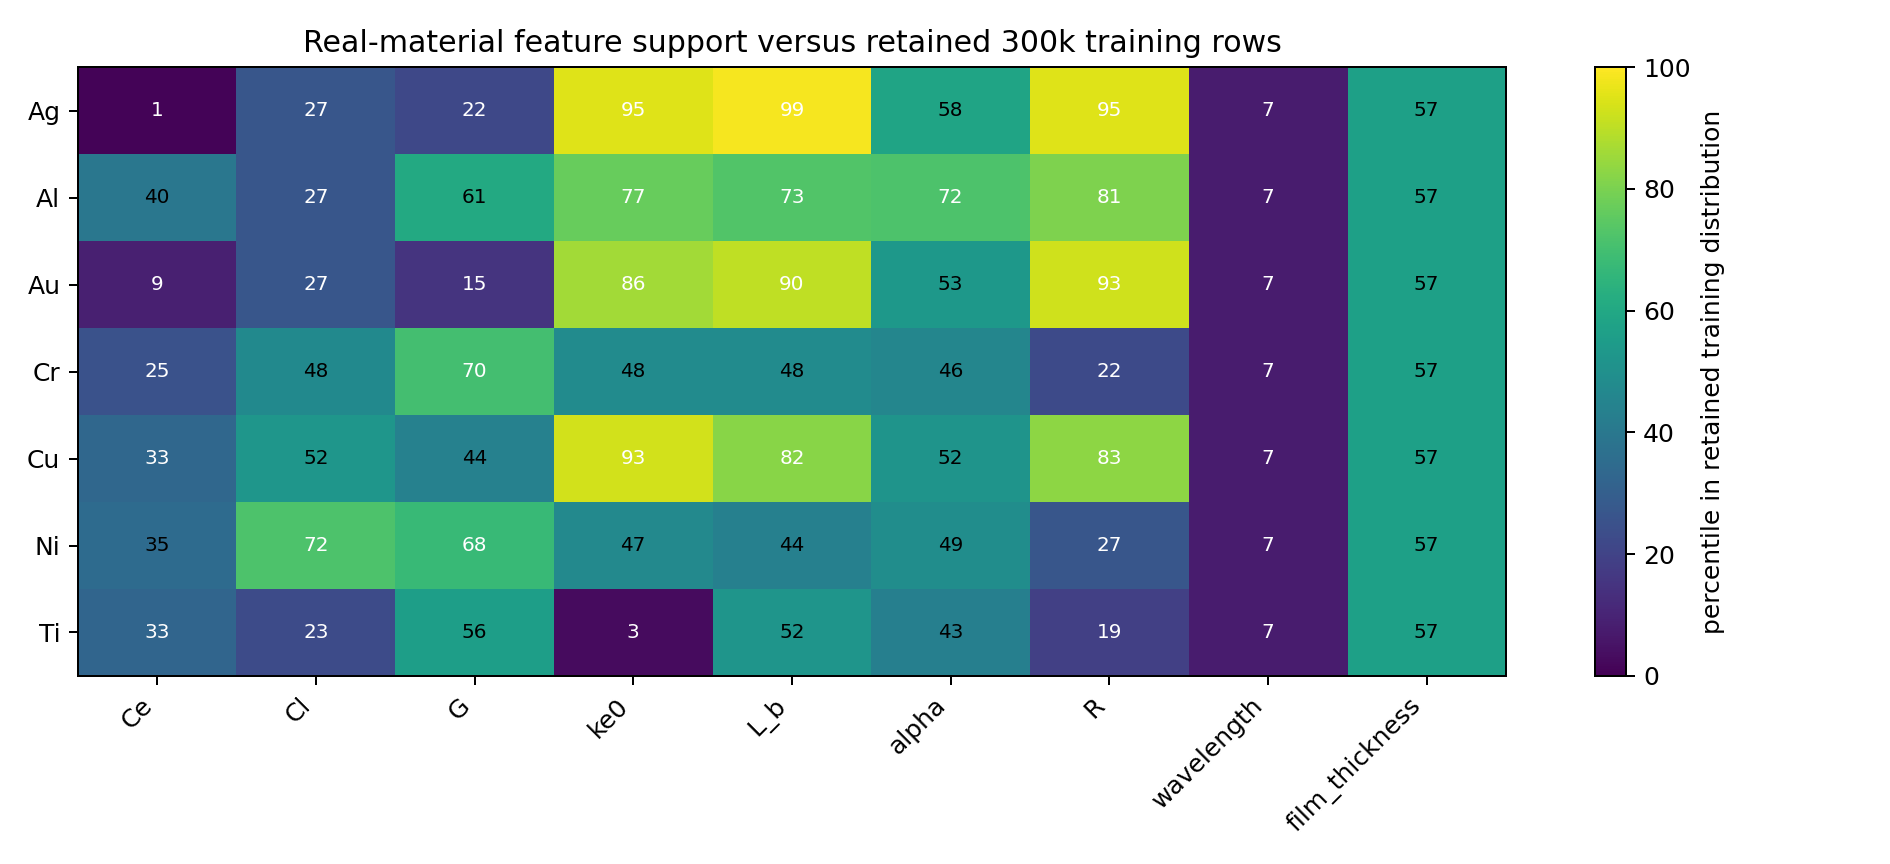
\includegraphics[width=0.92\textwidth]{figures/ch4/linear_ttm/material_feature_percentile_heatmap.png}
    \caption{Real-material feature support relative to the retained linear pTTM training distribution. Entries show the percentile location of each material parameter within the filtered synthetic dataset, so edge-percentile combinations identify material regimes where the retained surrogate manifold is less well supported.}
    \label{fig:ch4-material-feature-support}
\end{figure}

This pattern explains why the poor Cr, Ni, and Ti curve metrics in the linear experiment cannot be attributed simply to insufficient maximum sampled fluence. The synthetic fluence support spans $10$ to $40000\,\mathrm{J\,m^{-2}}$, so these cases are not outside the fluence interval used to construct the dataset. The dominant issue for the linear surrogate is instead that the training target policy censors high-temperature responses and that the retained filtered manifold does not fully support the material regimes reached by these curves. Increasing $F_{\max}$ alone is therefore not a sufficient correction unless the high-temperature target policy, sampling allocation, and acceptance strategy are also changed.

\section{Nonlinear pTTM extension}

The nonlinear extension replaces constant $C_e$ and $G$ by temperature-dependent thermophysical curves and replaces directly sampled optical source quantities by Lorentz--Drude descriptor sampling. A compact nonlinear input vector is
\begin{equation}
    \boldsymbol{\theta}_{\mathrm{nl}}
    =
    \left(
    \boldsymbol{\theta}_{\mathrm{scal}},
    \boldsymbol{\theta}_{\mathrm{LD}},
    \mathbf{c}^{C_e},
    \mathbf{c}^{G}
    \right),
\end{equation}
where $\boldsymbol{\theta}_{\mathrm{scal}}$ contains scalar thermal and geometric inputs, $\boldsymbol{\theta}_{\mathrm{LD}}$ contains optical descriptors, and $\mathbf{c}^{C_e}$ and $\mathbf{c}^{G}$ are spline coefficient vectors. The nonlinear lattice conductivity follows the same derived-quantity philosophy as the linear study, with $k_l=0.01\,k_e(T_e=T_l=\SI{300}{\kelvin})$.

For $Q\in\{C_e,G\}$, real-material thermophysical curves are fitted in log-space using a fixed open-clamped cubic B-spline basis \cite{cox1972numerical,deboor1972calculating,deboor1978splines}. Let $\boldsymbol{\tau}=(\tau_0,\ldots,\tau_{10})$ denote the knot vector and let $p=3$ be the degree. The zeroth-degree basis is
\begin{equation}
    B_{j,0}(T)
    =
    \begin{cases}
        1, & \tau_j\leq T<\tau_{j+1},\\
        0, & \mathrm{otherwise},
    \end{cases}
\end{equation}
and the higher-degree basis functions are given by the Cox--de Boor recursion
\begin{equation}
    B_{j,p}(T)
    =
    \frac{T-\tau_j}{\tau_{j+p}-\tau_j}B_{j,p-1}(T)
    +
    \frac{\tau_{j+p+1}-T}{\tau_{j+p+1}-\tau_{j+1}}B_{j+1,p-1}(T),
\end{equation}
where terms with zero denominator are omitted. The user-facing knot markers are
\begin{equation}
    [0,0,5,10,20,50,50]\,\mathrm{kK},
\end{equation}
which define the open-clamped cubic knot vector
\begin{equation}
    \boldsymbol{\tau}
    =
    [0,0,0,0,5,10,20,50,50,50,50]\,\mathrm{kK}.
\end{equation}
The endpoint repetitions clamp the spline at the temperature-domain boundaries. The internal knots at $\SI{5}{\kilo\kelvin}$, $\SI{10}{\kilo\kelvin}$, and $\SI{20}{\kilo\kelvin}$ mark changes in the local polynomial pieces.

\begin{figure}[htbp]
    \centering
    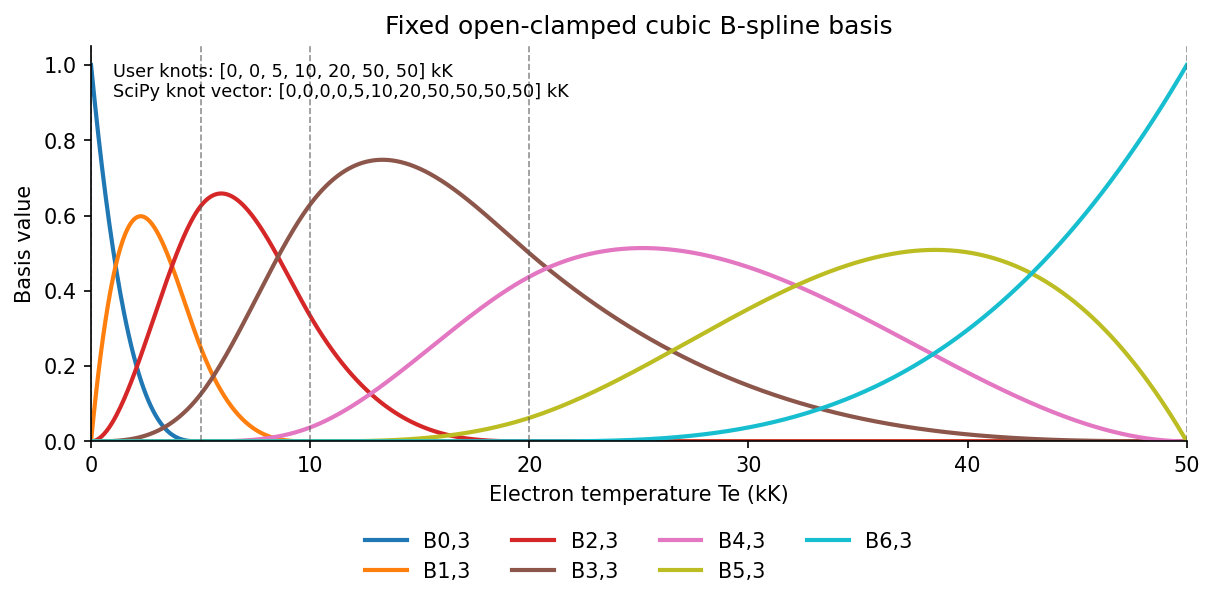
\includegraphics[width=0.86\textwidth]{figures/ch4/nonlinear_ttm/nonlinear_spline_basis_knots_no_greville.png}
    \caption{Fixed cubic B-spline basis used for the nonlinear thermophysical sampler. The vertical markers show the user-facing temperature knots that define the local polynomial intervals.}
    \label{fig:ch4-nonlinear-spline-basis}
\end{figure}

For a real material $m$ and property $Q$, the fitted log-spline coefficients solve the least-squares problem
\begin{equation}
    \mathbf{c}^{Q,m}
    =
    \arg\min_{\mathbf{c}\in\mathbb{R}^{7}}
    \sum_r
    \left[
        \log Q_m(T_r)
        -
        \sum_{j=0}^{6}c_j B_{j,3}(T_r)
    \right]^2.
\end{equation}
The fitted log curve is therefore
\begin{equation}
    \ell_Q(T)
    =
    \sum_{j=0}^{6}c_j^Q B_{j,3}(T),
    \qquad Q\in\{C_e,G\}.
\end{equation}
The physical thermophysical curve is reconstructed only after spline evaluation:
\begin{equation}
    Q(T)
    =
    \exp\!\left(\ell_Q(T)\right).
\end{equation}
This log-space construction is well suited to the present thermophysical sampling problem because $C_e(T)$ and $G(T)$ are strictly positive material properties. For any finite spline value $\ell_Q(T)$, exponentiation gives $Q(T)>0$ independently of the sign pattern of the coefficients. Positivity is therefore enforced by the reconstruction map rather than by clipping the physical curve or by imposing coefficient sign constraints. The finite-value check remains necessary because extreme sampled coefficients can still produce overflow or non-finite numerical evaluations.

The sampling distribution is defined coefficient-wise from the real-material fits. For each coefficient index,
\begin{equation}
    c_{j,\min}^{Q}
    =
    \min_m c_j^{Q,m},
    \qquad
    c_{j,\max}^{Q}
    =
    \max_m c_j^{Q,m}.
\end{equation}
The free coefficients are then sampled in the expanded log-coefficient envelope,
\begin{equation}
    c_j^Q
    \sim
    \mathcal{U}
    \left(
    c_{j,\min}^{Q}-1,\,
    c_{j,\max}^{Q}+1
    \right),
    \qquad j=0,\ldots,4.
\end{equation}
The high-temperature tail is constrained by
\begin{equation}
    c_5^Q=c_4^Q,
    \qquad
    c_6^Q=c_4^Q,
    \qquad Q\in\{C_e,G\}.
\end{equation}
Candidate curve pairs are accepted only when $C_e(T)$ and $G(T)$ are finite and strictly positive on the validation grid; invalid curves are rejected without clipping.

\begin{figure}[htbp]
    \centering
    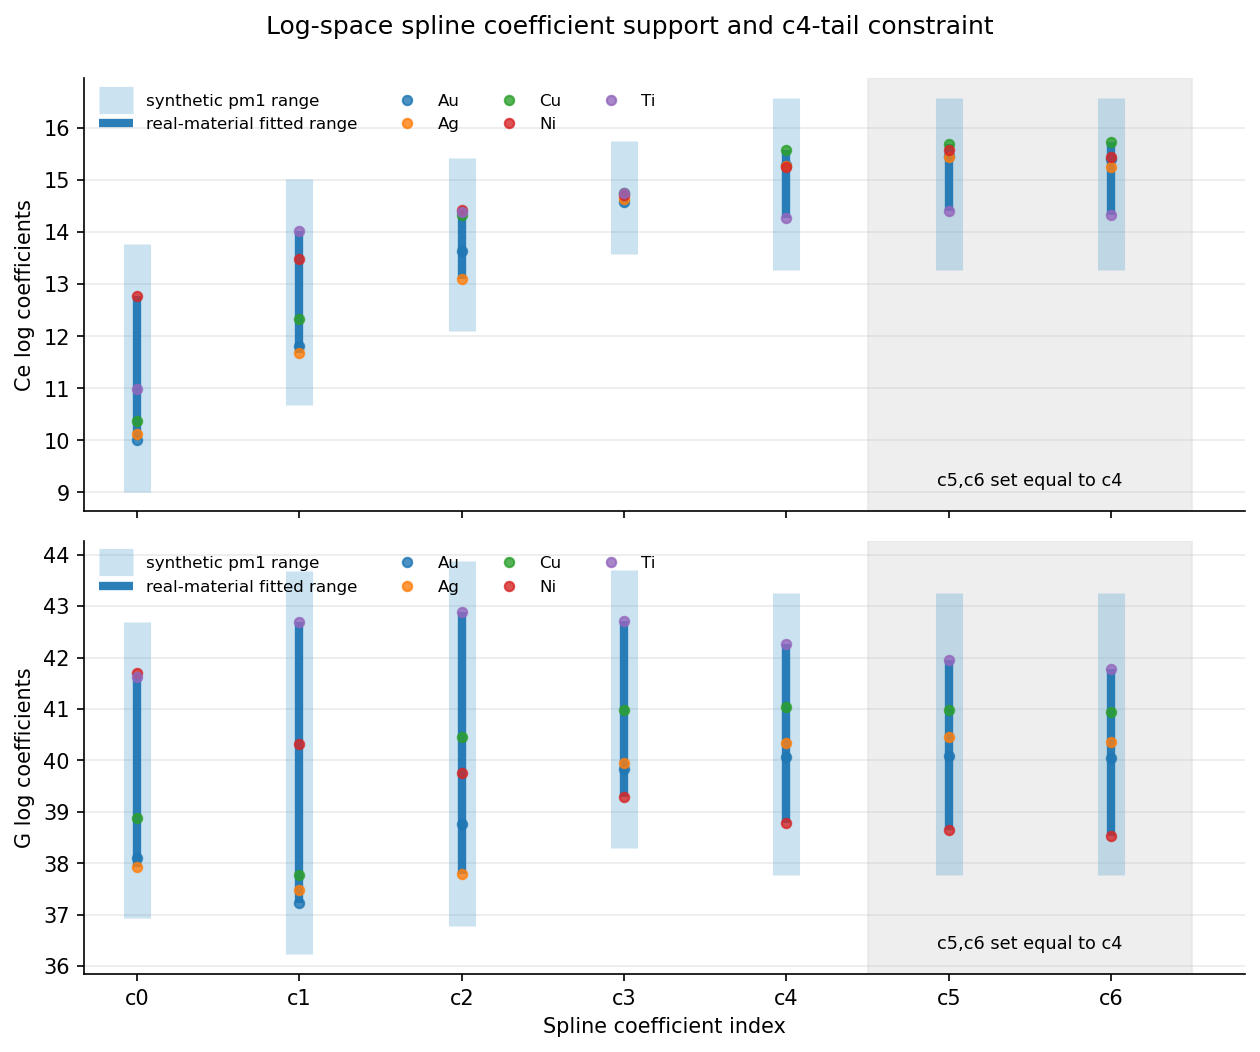
\includegraphics[width=0.90\textwidth]{figures/ch4/nonlinear_ttm/nonlinear_spline_coefficient_range_comb.png}
    \caption{Real-material and synthetic log-coefficient support for the nonlinear $C_e(T_e)$ and $G(T_e)$ splines. The narrow ranges show the fitted real-material coefficient envelope, while the wider ranges show the pm1 synthetic sampling envelope. The shaded tail region indicates the imposed $c_5=c_4$ and $c_6=c_4$ constraint.}
    \label{fig:ch4-nonlinear-spline-coefficient-comb}
\end{figure}

\begin{algorithm}[htbp]
    \caption{Spline-based nonlinear $C_e/G$ thermophysical sampling}
    \label{alg:ch4-nonlinear-ceg-sampling}
    \begin{algorithmic}[1]
        \Require Real-material curves $Q_m(T)$ for $Q\in\{C_e,G\}$, fixed cubic B-spline basis $\{B_{j,3}\}_{j=0}^{6}$
        \Ensure Accepted thermophysical curves $C_e(T)$ and $G(T)$
        \For{$Q\in\{C_e,G\}$}
        \For{each real material $m$}
        \State Fit log-space coefficients $\mathbf{c}^{Q}_{m}$ to $\log Q_m(T)$
        \EndFor
        \For{$j=0,\ldots,6$}
        \State Set $c^{Q}_{j,\min}\gets\min_m c^{Q}_{m,j}$ and $c^{Q}_{j,\max}\gets\max_m c^{Q}_{m,j}$
        \EndFor
        \For{$j=0,\ldots,4$}
        \State Draw $c_j^Q\sim\mathcal{U}(c^{Q}_{j,\min}-1,c^{Q}_{j,\max}+1)$
        \EndFor
        \State Set $c_5^Q\gets c_4^Q$ and $c_6^Q\gets c_4^Q$
        \State Reconstruct $Q(T)\gets\exp\!\left(\sum_{j=0}^{6}c_j^Q B_{j,3}(T)\right)$
        \EndFor
        \If{$C_e(T)$ and $G(T)$ are finite and strictly positive on the validation grid}
        \State Accept the curve pair
        \Else
        \State Reject the curve pair without clipping
        \EndIf
    \end{algorithmic}
\end{algorithm}

The nonlinear optical inputs are sampled as Lorentz--Drude descriptors, from which $\alpha$ and $R$ are derived at the sampled wavelength. This keeps the nonlinear extension closer to a material-response parameterisation than direct independent sampling of optical response scalars.

The nonlinear surrogate uses a source-term-informed feature set that augments the sampled scalar, Lorentz--Drude, and spline-coefficient descriptors with quantities motivated by the finite-thickness source normalisation. At room temperature, the ballistic-corrected absorption coefficient is
\begin{equation}
    \alpha_{\mathrm{eff},0}
    =
    \frac{\alpha_0}{1+\alpha_0 L_b},
\end{equation}
and the corresponding source-prefactor descriptor is
\begin{equation}
    \chi_{S,0}
    =
    \frac{
        \alpha_{\mathrm{eff},0}(1-R_0)
    }{
        1-\exp(-\alpha_{\mathrm{eff},0}h)
    }.
\end{equation}
The product
\begin{equation}
    F\chi_{S,0}
\end{equation}
couples the incident fluence to this effective source-prefactor scale. It is not the full volumetric source term, which also contains the spatial, temporal, and electromagnetic-envelope factors introduced in Chapter~\ref{ch:theoretical-background}. Appendix~\ref{app:ch4-sampling-support} gives the complete source-term-informed feature definitions, ranges, and correlation diagnostics.

\subsection{Nonlinear surrogate results}

The main-text nonlinear sampling diagnostic in Figure~\ref{fig:ch4-nonlinear-ceg-overlay} checks that exponentiating the accepted log splines produces positive thermophysical curves with broad real-material coverage. Additional real-material Lorentz--Drude descriptor distributions, nonlinear sampled marginals, derived marginals, feature definitions, and correlation diagnostics are collected in Appendix~\ref{app:ch4-sampling-support}.

\begin{figure}[htbp]
    \centering
    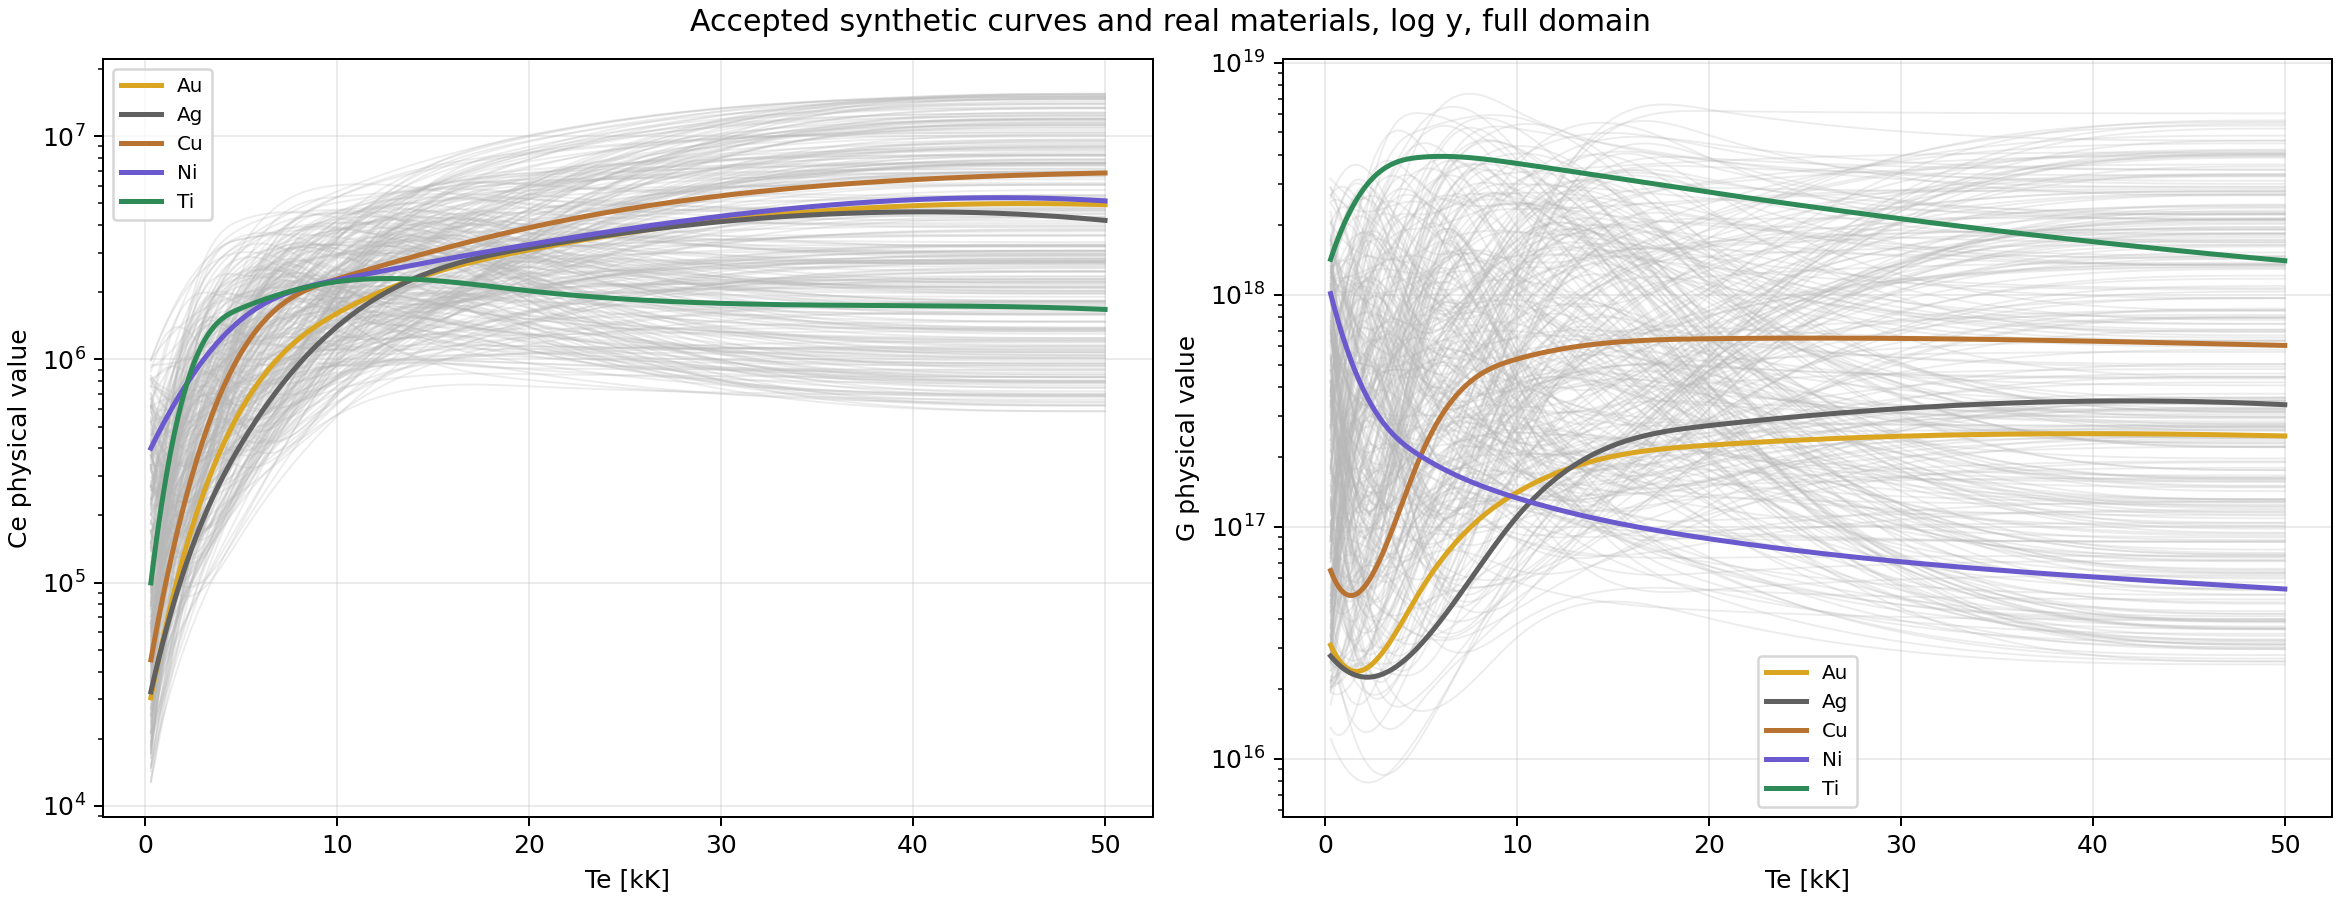
\includegraphics[width=0.92\textwidth]{figures/ch4/nonlinear_ttm/nonlinear_ce_g_spline_overlay.png}
    \caption{Accepted nonlinear $C_e(T_e)$ and $G(T_e)$ log-spline samples compared with the real-material curves used to define the coefficient envelope. The physical curves are obtained by exponentiating the evaluated log splines and rejecting non-finite or non-positive samples without clipping.}
    \label{fig:ch4-nonlinear-ceg-overlay}
\end{figure}

The nonlinear dataset was generated on a grid with \(N_x=101\), \(N_z=101\), and \(N_t=201\). It contains \(\num{20000}\) accepted samples from \(\num{22153}\) attempts; the remaining \(\num{2153}\) attempts were rejected because the solver diverged, terminated incompletely, or failed the accepted-sample checks. The deterministic 80/20 split gives \(\num{16000}\) training rows and \(\num{4000}\) held-out test rows.

At the outer-loop level, the nonlinear generation follows the accepted-sample template of Algorithm~\ref{alg:ch4-linear-data-generation}: candidate inputs are drawn, a pTTM solve is attempted, accepted rows are retained, and rejection reasons are recorded until the target sample count is reached. It is not, however, the same acceptance rule applied to a nonlinear solver. The linear study samples constant thermophysical and optical-source scalars and then applies the finite-response and \(T_{l,\max}\leq 10^4\,\mathrm{K}\) training filter. The nonlinear workflow first constructs Lorentz--Drude optical descriptors and log-spline \(C_e(T_e)\), \(G(T_e)\) curves, rejects non-finite or non-positive thermophysical curve pairs as in Algorithm~\ref{alg:ch4-nonlinear-ceg-sampling}, and then accepts a row only when the temperature-dependent nonlinear pTTM solve completes the required checks. The source-term-informed descriptors are computed from these sampled physical inputs before model training.

Table~\ref{tab:ch4-nonlinear-model-metrics} reports the held-out nonlinear surrogate metrics. LightGBM obtains an RMSE of \(\SI{376.449}{\kelvin}\), an MAE of \(\SI{158.066}{\kelvin}\), and \(R^2=0.96582\). The nonlinear MLP obtains an RMSE of \(\SI{276.836}{\kelvin}\), an MAE of \(\SI{149.760}{\kelvin}\), and \(R^2=0.98151\). Both nonlinear models use fixed bounded configurations; no full nonlinear Optuna hyperparameter optimisation was performed for the \(\num{20000}\)-sample analysis. The corresponding model-configuration table is kept in Appendix~\ref{app:ch4-sampling-support}, and large-scale nonlinear datasets should revisit full hyperparameter optimisation.

\begin{table}[htbp]
    \centering
    \caption{Held-out synthetic test metrics for the 20,000-sample nonlinear 2D pTTM surrogate analysis.}
    \label{tab:ch4-nonlinear-model-metrics}
    \small
    \begin{tabular}{lrrrrr}
\toprule
Model & Train rows & Test rows & RMSE (K) & MAE (K) & $R^2$ \\
\midrule
LightGBM & 16000 & 4000 & 376.449 & 158.066 & 0.96582 \\
MLP & 16000 & 4000 & 276.836 & 149.760 & 0.98151 \\
\bottomrule
\end{tabular}

\end{table}

The material-validation results show why the nonlinear analysis changes the interpretation of the earlier transition-metal failures. In the nonlinear validation, Ni is predicted strongly, with \(R^2=0.9864\) for LightGBM and \(R^2=0.9883\) for the MLP. Ti is also strong, with \(R^2=0.9930\) for LightGBM and \(R^2=0.9765\) for the MLP. These results improve substantially on the corresponding linear failure cases. Ag, Au, and Cu show more mixed nonlinear surrogate transfer, so they should be interpreted as evidence that material support and threshold inversion remain sensitive even when the nonlinear thermophysical model is included, especially at this limited sample size. Cr and Al are excluded from the nonlinear comparison because compatible material-specific nonlinear \(C_e(T_e)\) and \(G(T_e)\) curves were unavailable. The complete material-validation table is given in Appendix~\ref{app:ch4-sampling-support}.

\begin{figure}[htbp]
    \centering
    \subfloat[Ni validation curve.\label{fig:ch4-nonlinear-ni-validation}]{%
        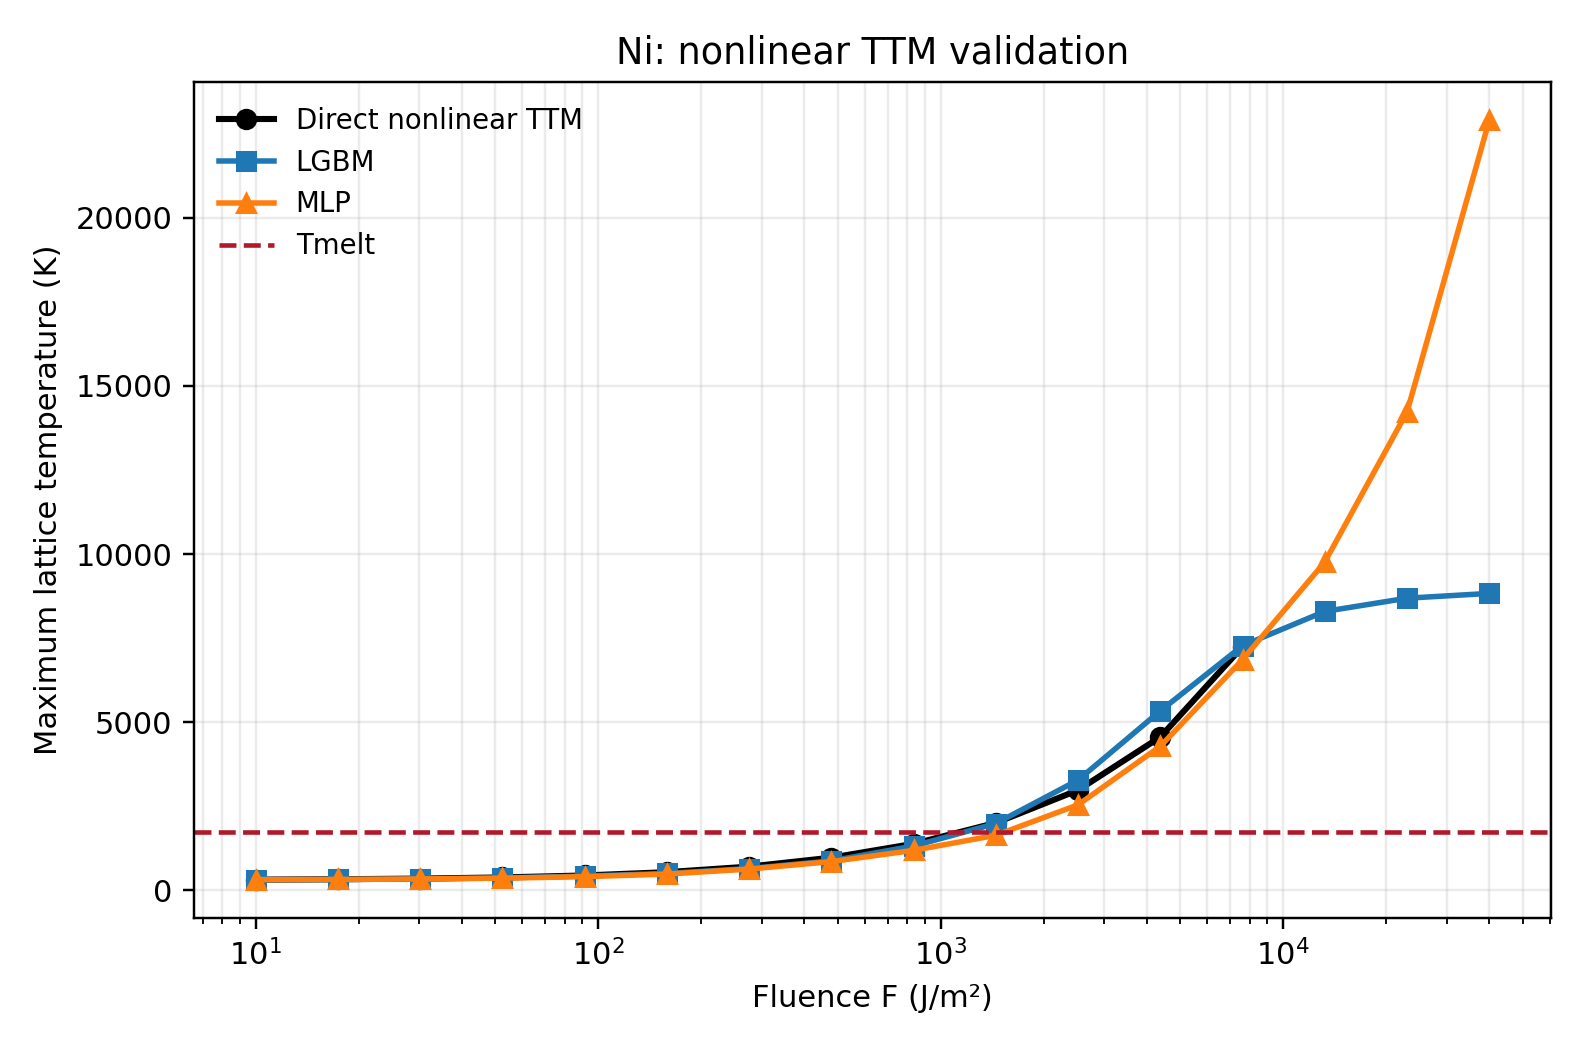
\includegraphics[width=0.48\textwidth]{figures/ch4/nonlinear_ttm/final_20k/nonlinear_Ni_validation.png}
    }
    \hfill
    \subfloat[Ti validation curve.\label{fig:ch4-nonlinear-ti-validation}]{%
        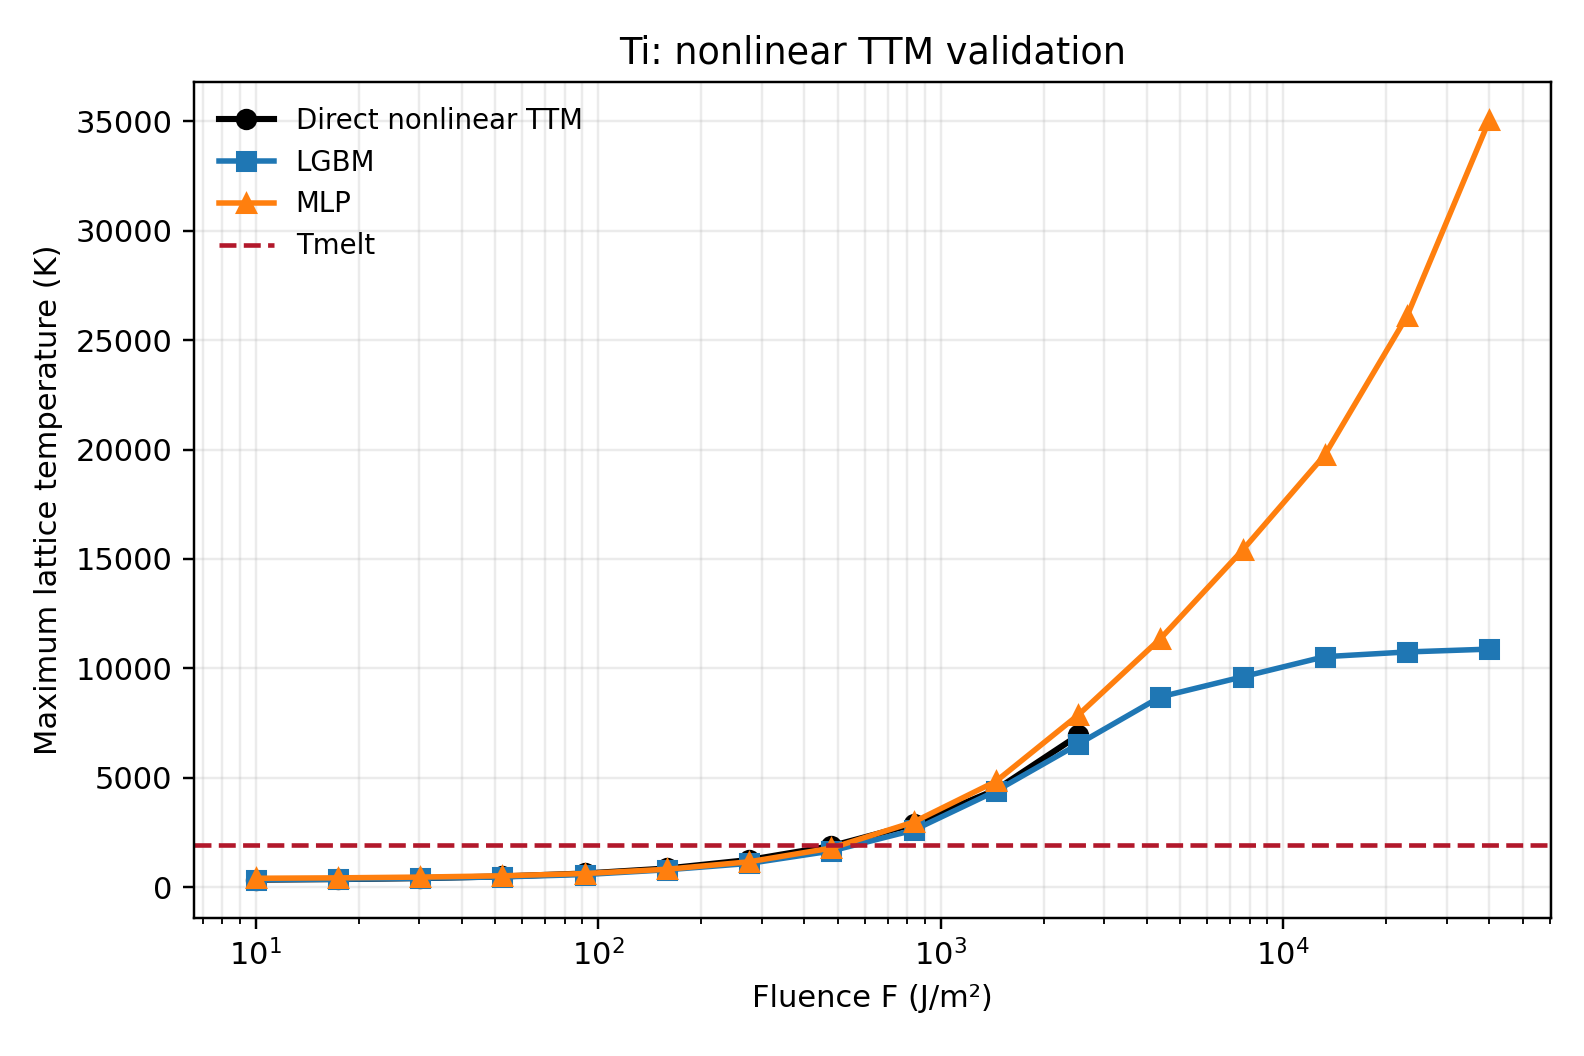
\includegraphics[width=0.48\textwidth]{figures/ch4/nonlinear_ttm/final_20k/nonlinear_Ti_validation.png}
    }
    \caption{Nonlinear 20,000-sample material-validation overlays for the source-term-informed LightGBM and MLP surrogates. Supplementary Ag/Au/Cu overlays and the full material-validation table are collected in Appendix~\ref{app:ch4-sampling-support}.}
    \label{fig:ch4-nonlinear-ni-ti-validation}
\end{figure}

The direct nonlinear threshold calculations and surrogate inversions are reported without external cross-model values. The Ni and Ti behaviour is closer to the nonlinear internal reference scale than in the earlier linear failure case, while threshold inversion remains imperfect for some materials.

\begin{table}[htbp]
    \centering
    \caption[Nonlinear threshold comparison omitted]{External threshold comparison values omitted from public source pending redistribution terms.}
    \label{tab:ch4-external-threshold-comparison}
    \scriptsize
    \PublicExternalValuesOmitted[0.82\textwidth]
\end{table}

\begin{figure}[htbp]
    \centering
    \PublicExternalValuesOmitted[0.82\textwidth]
    \caption[Nonlinear threshold comparison omitted]{External threshold comparison values omitted from public source pending redistribution terms.}
    \label{fig:ch4-nonlinear-threshold-comparison}
\end{figure}

The target-tail limitation observed in the linear surrogate should therefore be interpreted as a limitation of that specific linear surrogate experiment, rather than as a general explanation for all refractory or transition-metal behaviour. The nonlinear \(\num{20000}\)-sample study is also an accepted-sample study: divergent or incomplete simulations were rejected, and accepted lattice-temperature maxima remained below approximately \(10^4\,\mathrm{K}\). Nevertheless, the nonlinear Ni and Ti validation curves improve substantially relative to the linear failure case. This indicates that the earlier poor behaviour cannot be attributed to fluence range or target censoring alone. In the nonlinear study, the remaining limitations are better described as a combination of the small accepted-sample regime, material-data availability, the support of the source-term-informed feature set, and surrogate threshold-inversion error.

\section{Limitations and future work}

The principal limitation of the linear surrogate study is target-tail censoring. The $T_{l,\max}\leq\SI{10000}{\kelvin}$ cap makes the retained regression task stable and interpretable, but it also excludes the high-temperature part of the numerical response where several transition-metal validation curves fail. Future linear datasets should therefore include an explicit high-temperature-tail policy, for example through stratified sampling, active learning near the cap, or a separate regime-specific model rather than by increasing the fluence range alone.

The nonlinear analysis reduces some of the earlier material-transfer failures, especially for Ni and Ti, but it does not remove all limitations. It is still a \(\num{20000}\) accepted-sample study with practical solver-acceptance limits, fixed bounded model configurations, and imperfect threshold inversion. Large-scale nonlinear datasets remain future work, together with full nonlinear hyperparameter optimisation, prediction-interval calibration for the nonlinear target, and multi-target learning of \((T_{l,\max},\tau_{\mathrm{eq}})\).

Cr and Al are excluded from the nonlinear validation because compatible material-specific nonlinear \(C_e(T_e)\) and \(G(T_e)\) curves were unavailable. Future nonlinear validation should therefore extend the thermophysical database used for surrogate construction and real-material comparison.

External cross-model threshold values are omitted from this public source pending documented redistribution terms. The residual-calibrated intervals reported for the linear study quantify held-out surrogate residuals relative to the numerical linear pTTM target only. Numerical-solver uncertainty and material-parameter uncertainty remain outside the present evidence base.

The optical-source model should also be extended for metallic thin films below approximately \(\SI{200}{\nano\metre}\), where finite-film effects can overlap with the ballistic-transport length scale. The present pTTM source incorporates ballistic and finite-thickness Beer--Lambert corrections, but it does not model coherent rear-interface reflection or finite-film transmission. A suitable next step is a multiple-reflection formulation based on the closed-form Airy solution for a single ambient/metal/substrate stack, equivalently the single-film transfer-matrix expression, to obtain the reflectance, transmittance, and absorptance used to normalise the laser source \cite{Tsibidis_Mansour_Stratakis_2022}. For highly reflective metals, this closed-form expression is preferable to a truncated Born reflection series, whose round-trip contribution may converge too slowly to be useful. Any such extension should specify the substrate optical properties and quantify its effect on both direct pTTM thresholds and the synthetic data used for surrogate training.
